\newpage
\section{Word相关操作}
\subsection{公式排版相关知识}
在数学上,一般规定,字母(包括角标上的字母)作为变量时用斜体,不是变量时用直立体(正体)。

比如$x^2+x+1=0$这里的字母$x$是变量,就是斜体。$x=\frac{-1\pm{}\sqrt{3}\mathrm{i}}{2}$中$\mathrm{i}$不是变量,用直立体。
另外,自然常数$\mathrm{e}$和圆周率$\uppi$还有微分符号$\mathrm{d}$都不是变量,用直立体。以及热力学中$\Delta{}T_{ab}$的角标表示的是a点和b点,也不是变量,用直立体,这里的$\Delta$也是直立体。

除此之外,在数学规定的基础上,热力学中状态函数和相关物理量如$H$、$G$、$S$、$T$、$P$、$V$、$n$等都用斜体。在化学分子式中,字母和数字都是直立体。

Word的公式编辑器会默认所有字体全都是斜体的,有时候需要自己手动更改为直立体。

\subsection{WPS}
\subsubsection{WPS优缺点}
尽量不要使用WPS!!!很多时候WPS会造成莫名其妙的混乱,请尽量不要使用。

WPS可能有很多内置模板,方便使用。并且学校也购买了正版,可以直接使用。
另外,WPS提供教育版,免费无广告,也可下载使用。

如果只是个人使用,无需与其他人交互,不向外共享文件,或转换成PDF共享,
幻灯片也只在自己电脑上放映,WPS还是不错的。
但是很多时候都会遇到兼容性问题。
特别是专业领域,如插入数学公式,或者ChemDraw图形,WPS很难胜任。

\subsubsection{使用MS Office} 

另外如果你购买的是带有系统的品牌电脑,售价的一部分是包括MS Office家庭版的,
可以直接打开使用,并无需付费。
如果你的品牌机赠送的是Office365一年或两年订阅,使用期过后,
也可到\textbf{\textcolor{blue}{\href{https://zbhrj1.jlu.edu.cn/download/office2021.html}{吉大正版网站}}}下载使用。

\subsection{Word模板使用}
\textbf{此部分请自行操作体会}:
Word模板文件通常以.dotx为后缀,双击即可新建文档。\textbf{注意}此时是新建文档,
并不是编辑模板文件,只是以模板文件为基础新建一个文档。
\textbf{可先另存为到本地,之后再进行编辑。}

\subsection{Word标题格式}

我提供的模板文件中已经设置了标题格式,直接使用即可。
另外,\textbf{标题无需手动编号},已设置自动编号:

\begin{figure*}[!h]
    \captionsetup{font={small, bf}, margin=60pt}
    \centering
    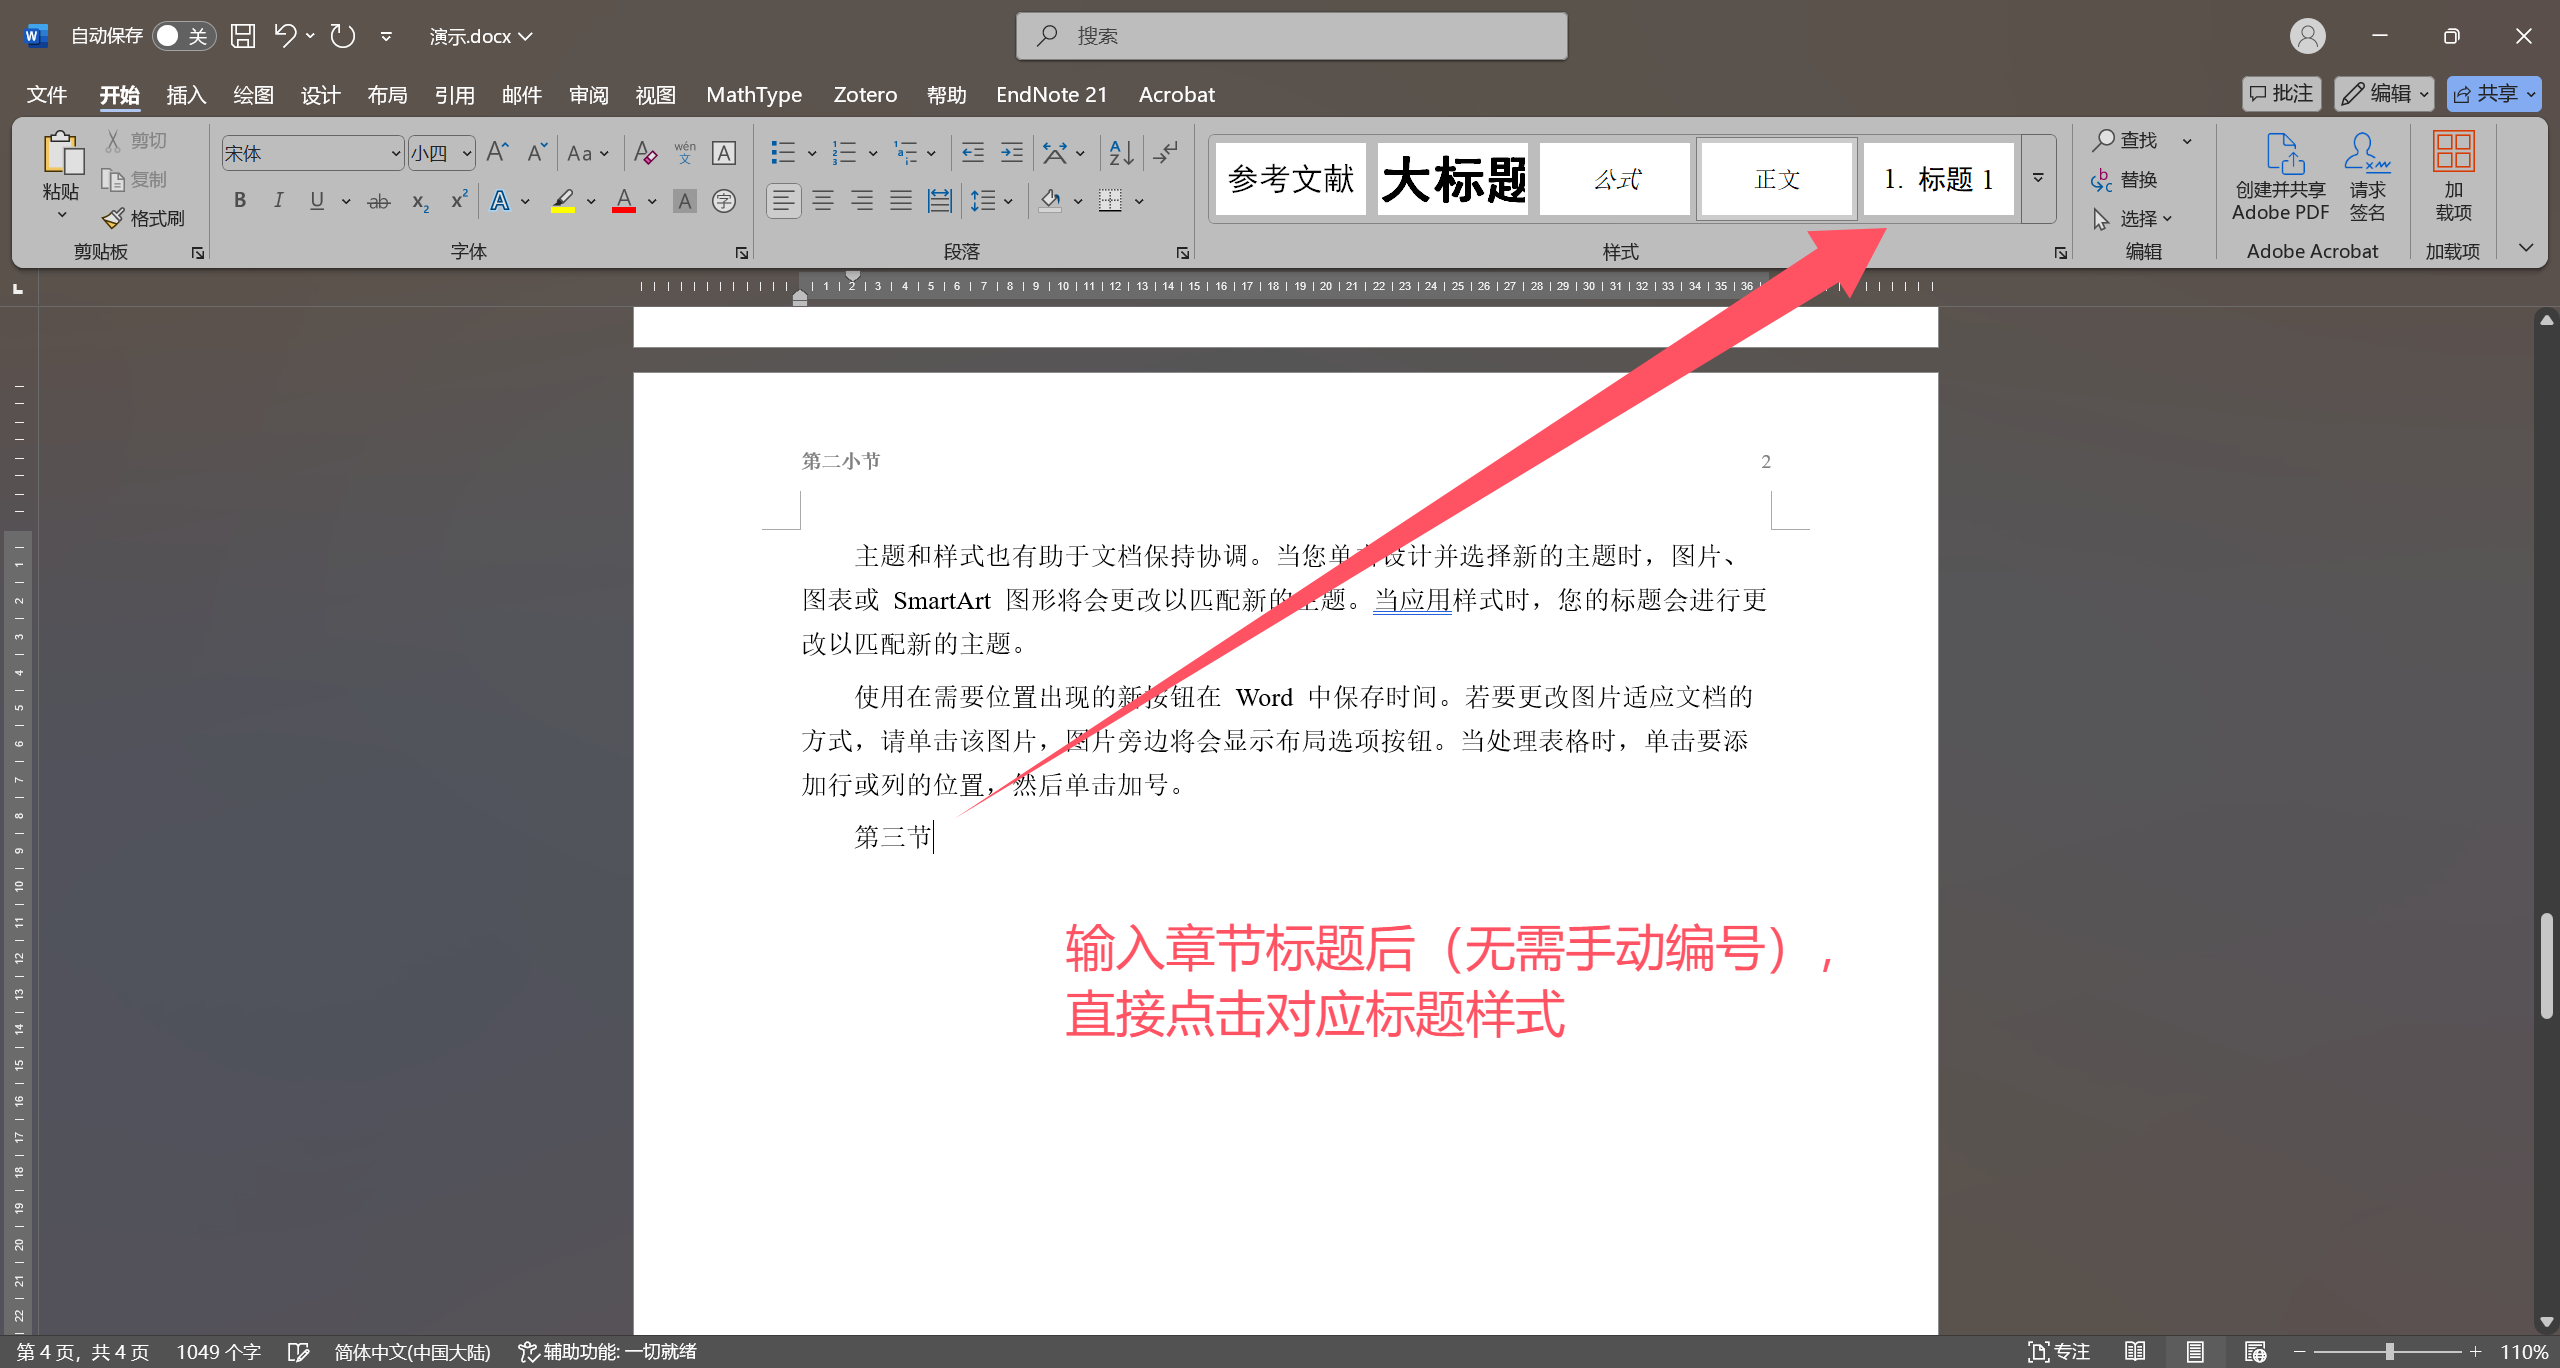
\includegraphics[width=\textwidth]{模板标题.png}
\end{figure*}
\begin{figure}[!h]
    \captionsetup{font={small, bf}, margin=60pt}
    \centering
    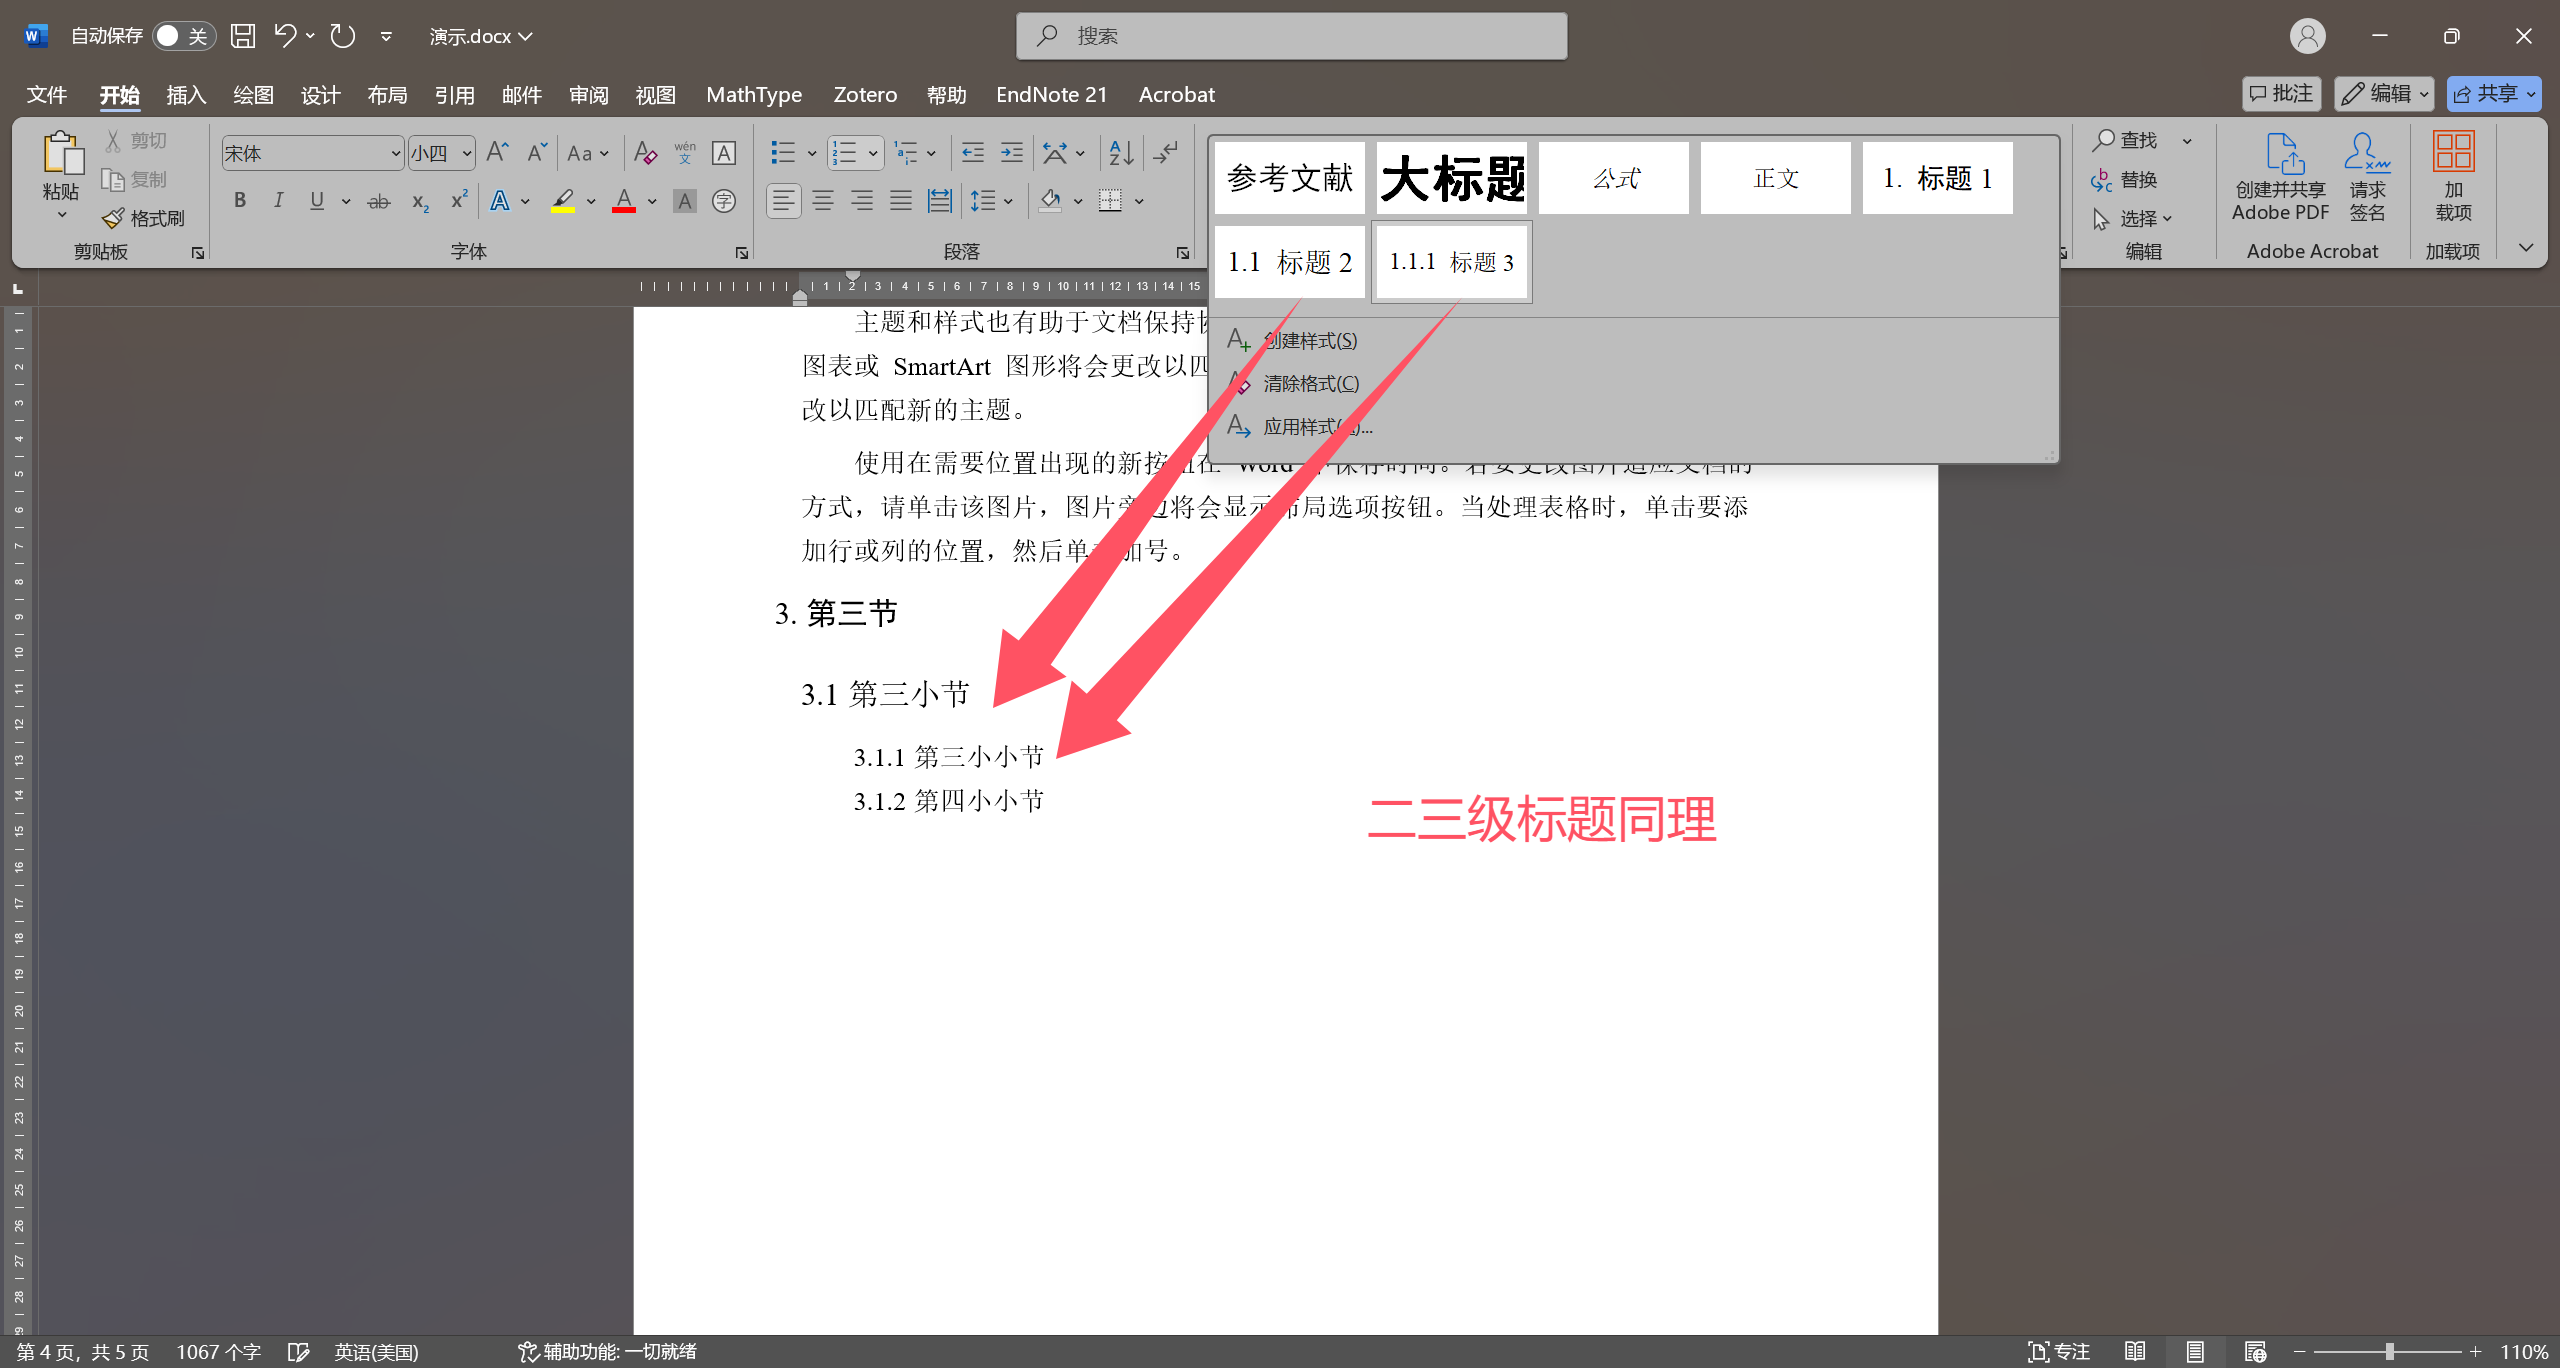
\includegraphics[width=\textwidth]{模板标题2.png}
    \caption{模板标题}
    \label{Word 2}
\end{figure}

\newpage

\subsection{目录}

我这个模板已经添加了目录,但它是不会自动更新的,

在添加新章节后,可以到“引用”选项卡,点击“更新目录”,
选择“更新整个目录”,即可更新目录:
\begin{figure}[!h]
    \centering
    \captionsetup{font={small, bf}, margin=60pt}
    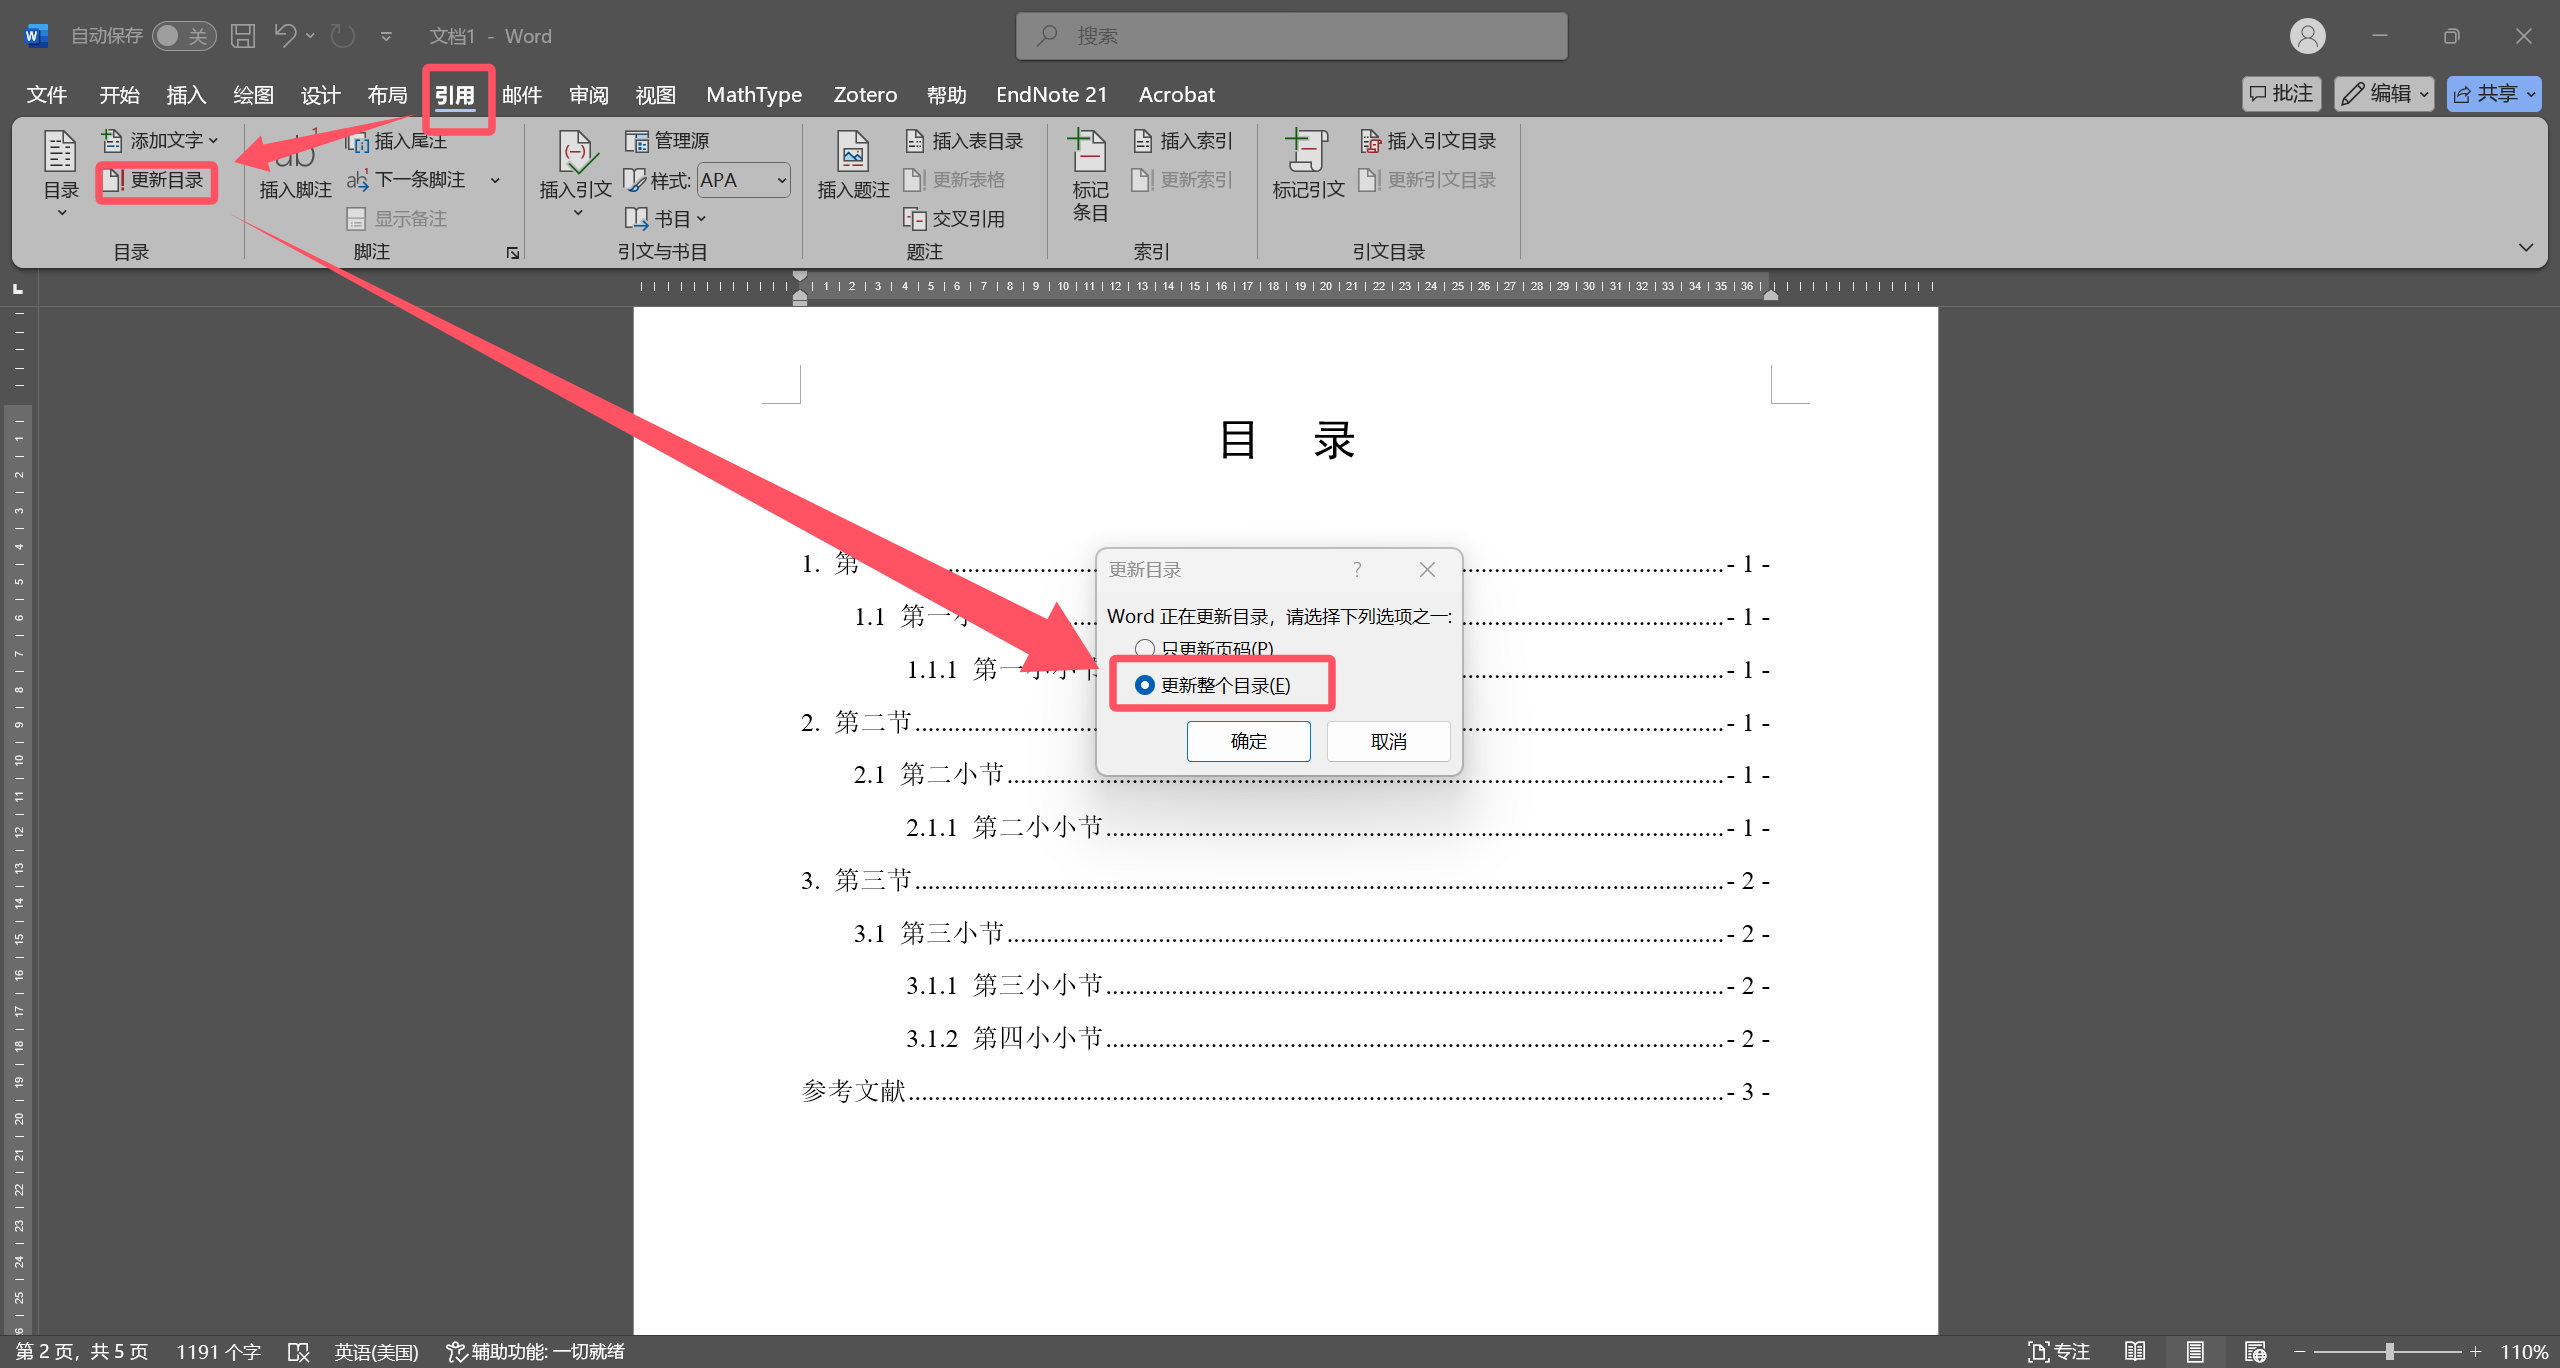
\includegraphics[width=\textwidth]{更新目录.png}
    \caption{更新目录}
    \label{Word 3}
\end{figure}

\subsection{在WPS中使用}
\subsubsection{WPS专业版下载}
我下载了多种WPS版本测试,发现专业版能够较好地兼容Zotero和公式,其它版本的WPS若没有启用宏,则无法使用Zotero。
学校购买了WPS专业版正版,可以在\textbf{\textcolor{blue}{\href{https://zbhrj1.jlu.edu.cn/download/wpsp.html}{吉大正版网站}}}直接下载使用。
在网站上有详细安装步骤,这里不再赘述。

注意安装时,可以更改安装路径,比如安装在“D:\backslash{}Kingsoft\backslash{}WPS Office”文件夹下。
另外,如果平时还是使用MS Office为主,可以在安装页面取消相关格式关联,或者在安装后也能在设置里更改。

\textbf{注意:在“WPS文字”中,大部分操作与Word相同,但有些操作会有所不同,在下面只介绍不同部分。}

\subsubsection{在WPS使用模板}
我提供的模板在WPS中也能使用,右击此模板文件,选择用“WPS文字”打开即可:
\begin{figure}[!h]
    \centering
    \captionsetup{font={small, bf}, margin=60pt}
    \begin{subfigure}[c]{0.9\textwidth}
    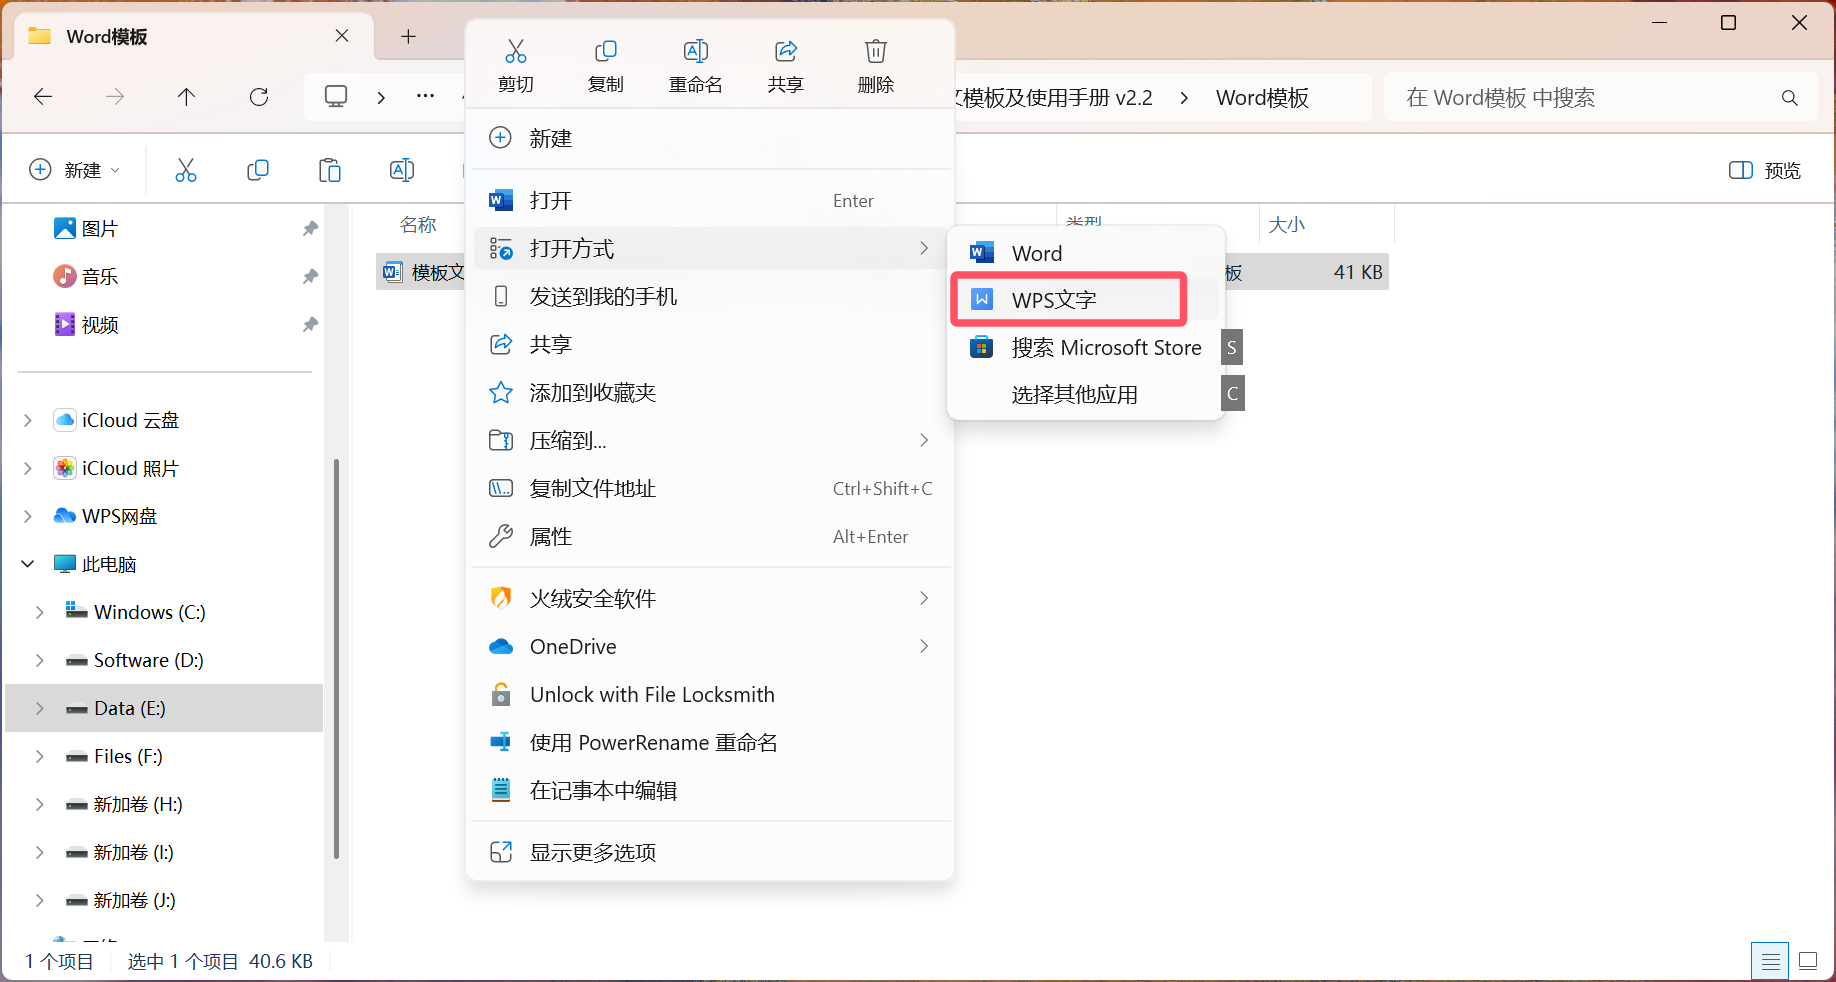
\includegraphics[width=\textwidth]{用WPS打开模板文件.png}
    \end{subfigure}    
    \caption{用WPS打开模板文件}
    \label{WPS 1}
\end{figure}

在WPS文字插入公式时,与Word不同的是,WPS默认所有字母和文字为正体,需要手动将一些字母改为斜体。可以选中后按快捷键Ctrl+I,快速切换正体与斜体。

另外,WPS内置了很多样式,下图里我把我模板里带的样式框起来了,与Word中一一对应,其中红色是使用得到的样式,操作方法与Word中相同:

\begin{figure}[!h]
    \centering
    \captionsetup{font={small, bf}, margin=60pt}
    \begin{subfigure}[c]{0.9\textwidth}
    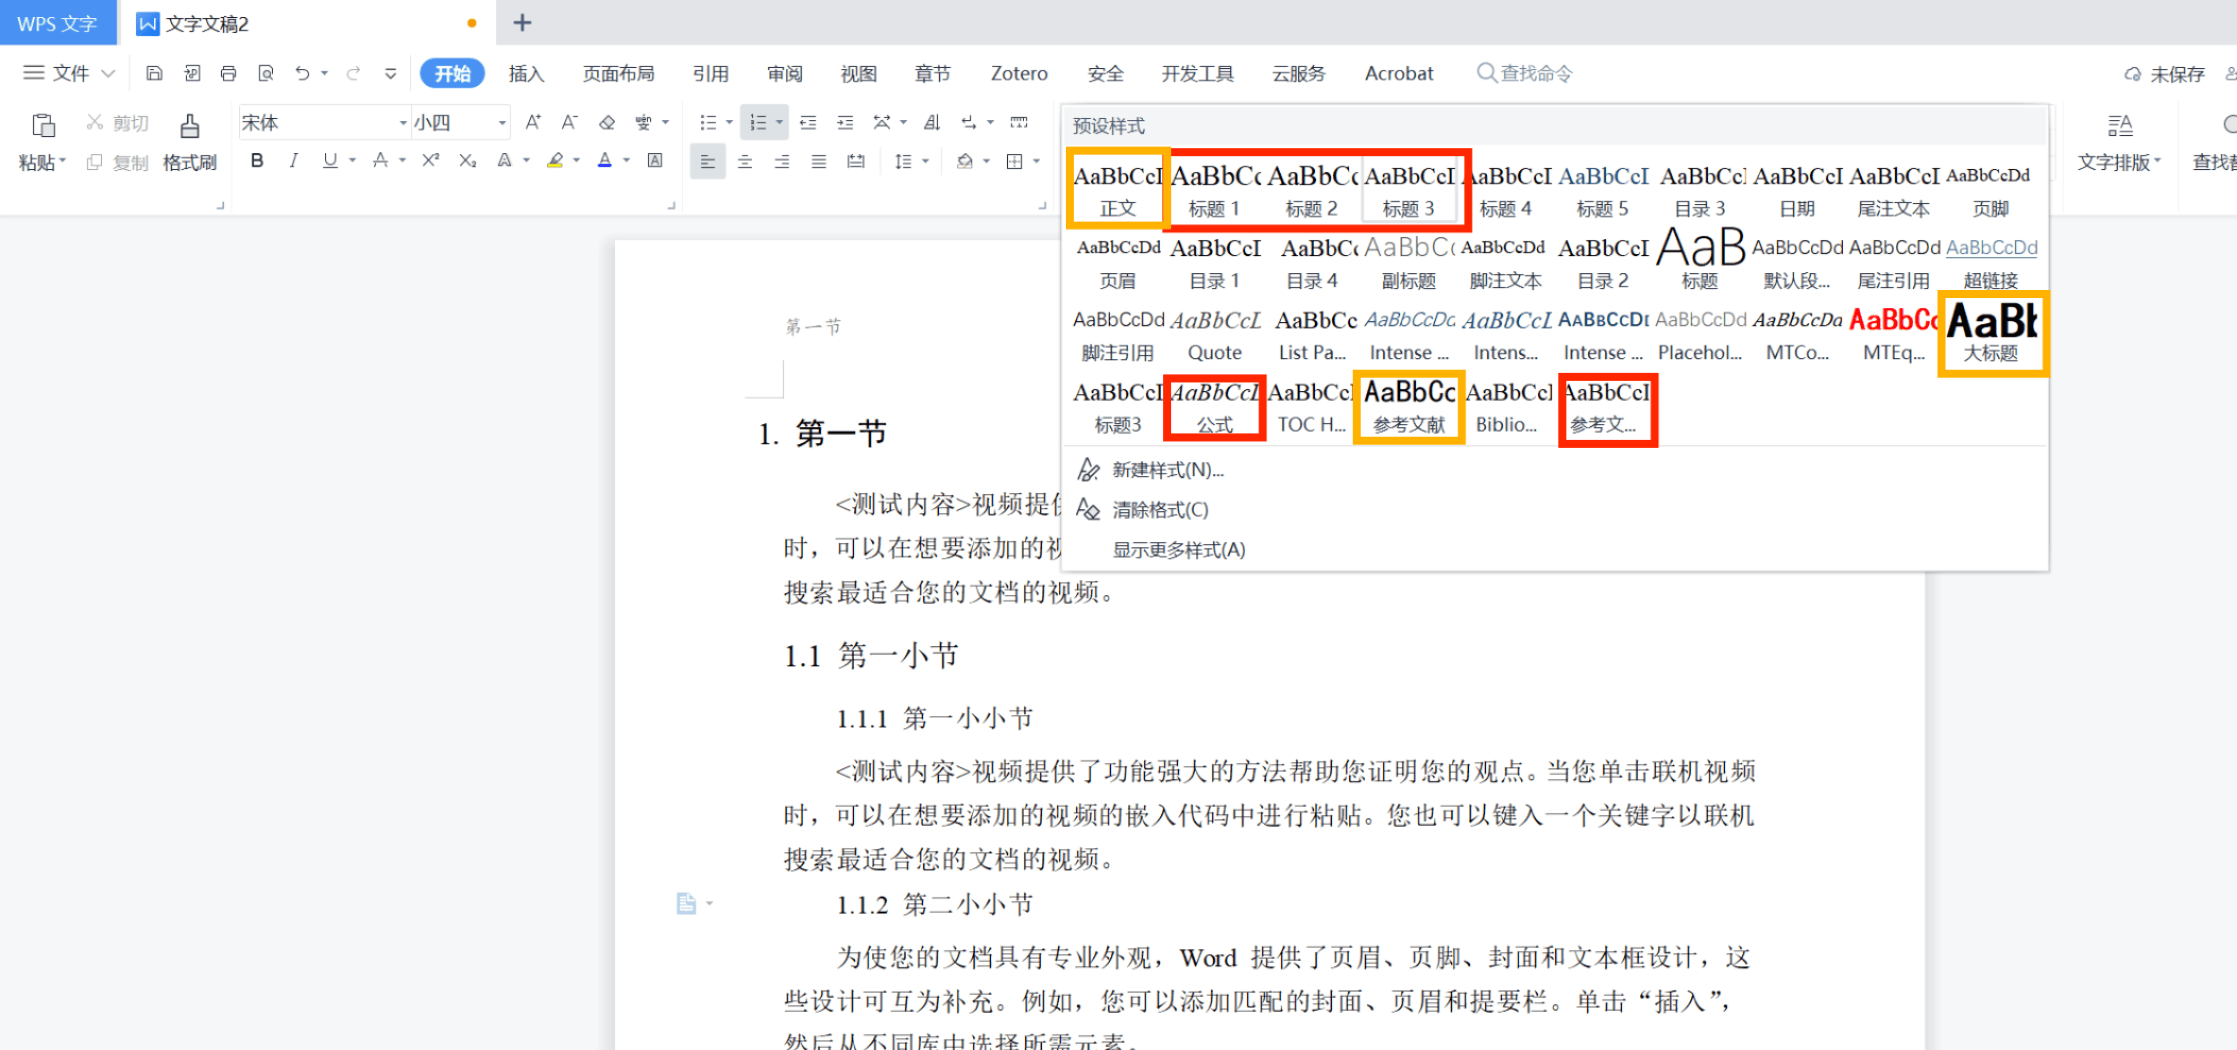
\includegraphics[width=\textwidth]{模板里的样式.png}
    \end{subfigure}    
    \caption{模板的样式}
    \label{WPS 2}
\end{figure}

\subsubsection{导出为PDF}

按下图所示,点击导出为PDF,检查输出路径和导出选项无误,即可导出:
\begin{figure}[h]
    \centering
    \captionsetup{font={small, bf}, margin=60pt}
    \begin{subfigure}[c]{0.6\textwidth}
      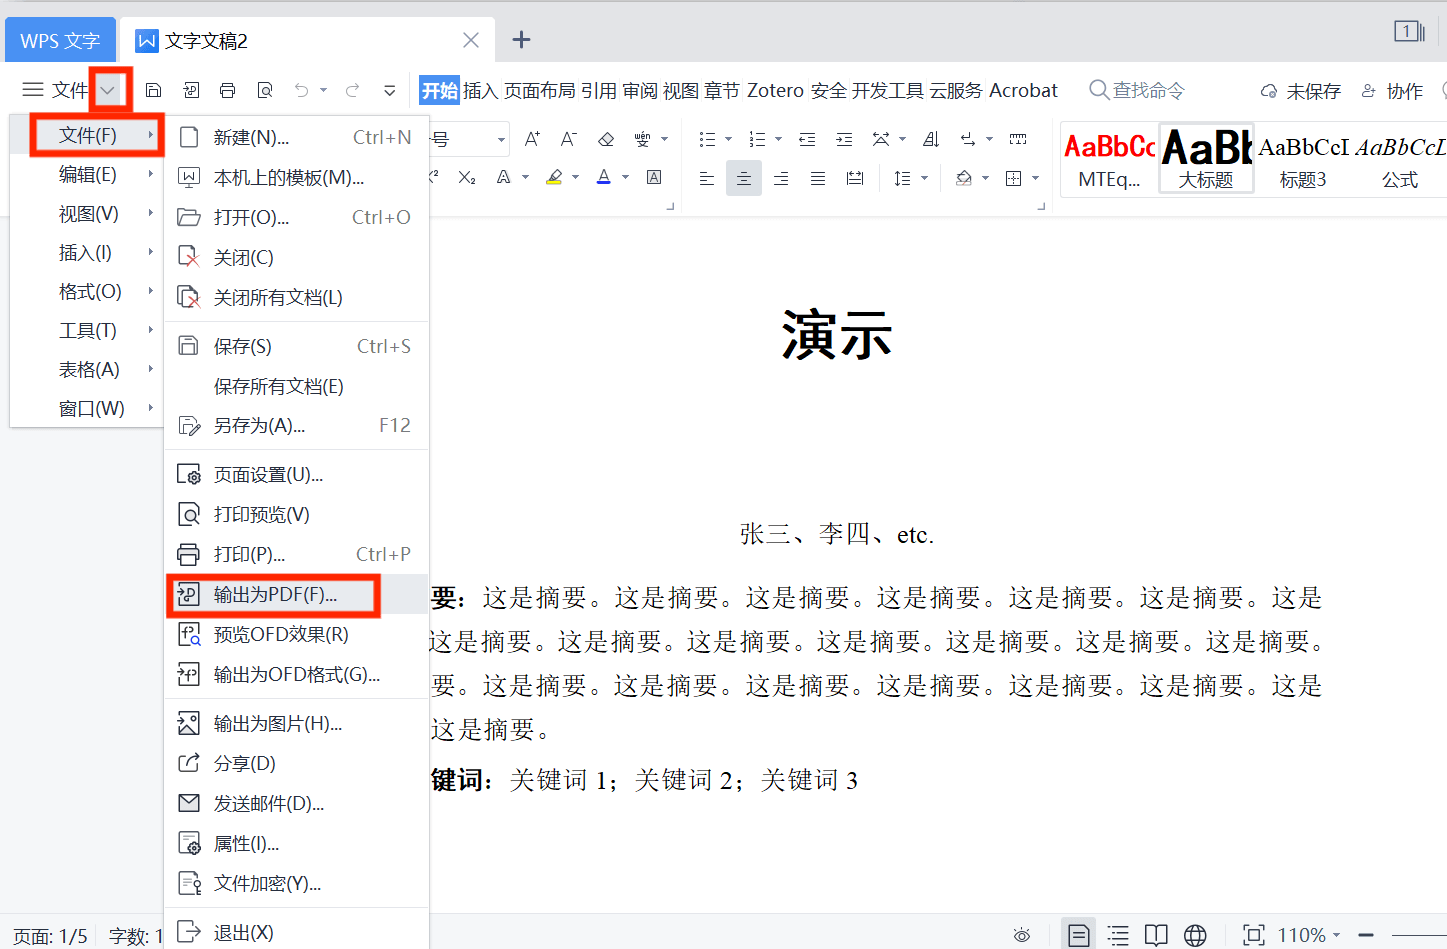
\includegraphics[width=\textwidth]{WPS导出为PDF.png}
    \end{subfigure}
    \hfill
    \begin{subfigure}[c]{0.35\textwidth}
      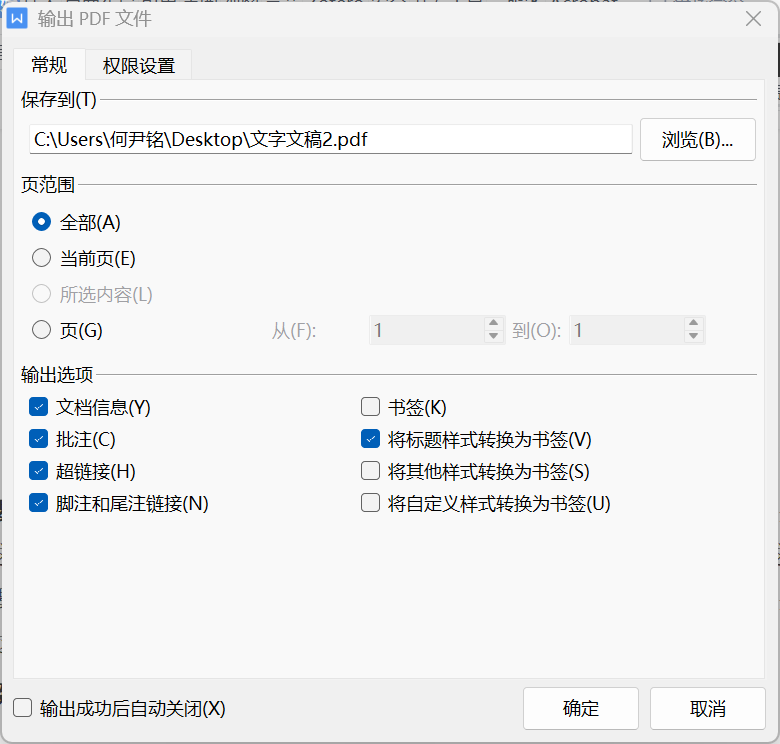
\includegraphics[width=\textwidth]{检查导出选项.png}
    \end{subfigure}
    \caption{WPS导出为PDF}
    \label{WPS 3}
\end{figure}

\subsection{碎碎念}
首行缩进2字符不要用空格!!!就算于吉红这么写我都照样骂(虽然她可能不在意就是了=\_=)。
本模板“正文”样式已经设置了首行缩进,也不需要手动设置。

这只是个很简陋的模板,但基本够用。
如果你有一定的Word基础,可以跟据自己喜好调整修改样式。

如果你对Word不熟悉,或者不想折腾,可以直接使用我这个模板。

希望我这个模板能带来一些帮助。
但事实上,用Word排版是远远不够的,
你在写论文时,如果遇到插入图片、图表,稍加调整,整篇文章可能就乱了。

不过,它所见即所得的编辑模式,对刚接触电脑的人很友好。
而且,如果你对Word十分熟悉,上面所提到的问题也都能解决,不过学习成本较高。

所以接下来,我将介绍更加专业的排版工具:\LaTeX。